\documentclass[a4paper,twoside,10pt]{book}
% PAGE DIMENSIONS
% FOR A5 without scaling
%\usepackage[inner=18mm, outer=10mm,top=20mm,headsep=10mm,bottom=10mm,paperwidth=148mm,paperheight=210mm]{geometry}
% FOR 17x24cm
\usepackage[inner=30mm, outer=20mm,top=24mm,headsep=10mm,bottom=20mm,paperwidth=170mm,paperheight=240mm]{geometry}
% FOR A4
%\usepackage[inner=50mm, outer=40mm,top=60mm,headsep=10mm,bottom=57mm,paperwidth=210mm,paperheight=297mm]{geometry}
%\usepackage[inner=8.5mm, outer=12.5mm,top=10mm,headsep=5mm,bottom=10mm,paperwidth=141mm,paperheight=200mm]{geometry}
%\usepackage[inner=30mm, outer=23mm,top=29mm,headsep=10mm,bottom=23mm,paperwidth=210mm,paperheight=297mm]{geometry}
% FOR A5
%\usepackage[inner=25mm, outer=17mm,top=8mm,headsep=8mm,bottom=17mm,paperwidth=148mm,paperheight=210mm,includehead]{geometry}
% TABLES: full-width using X{10cm} column
\usepackage{tabularx}
% DRAWINGS (for chapter title)
\usepackage{tikz}
% TYPOGRAPHY: 
\usepackage[protrusion=true,final,factor=1500]{microtype}

% SOME extra math symbols
\usepackage{amssymb}




% CAPTIONS of figures/table styling
\usepackage[font={stretch=1.1,small},labelfont=bf]{caption} % order matters: stretch, then size
%\usepackage[font={small,sf},labelfont=bf]{caption} % small sans-serif + bold

% FONT  SIZES
\usepackage{fix-cm} % FOR ANY font sizes, not predefined
\renewcommand\footnotesize{\fontsize{7pt}{7pt}\selectfont}
\renewcommand\small{\fontsize{6pt}{6pt}\selectfont}
\renewcommand\normalsize{\fontsize{9pt}{9pt}\selectfont}
\renewcommand\large{\fontsize{10pt}{10pt}\selectfont}
\renewcommand\Large{\fontsize{11pt}{11pt}\selectfont}
\renewcommand\Huge{\fontsize{24pt}{24pt}\selectfont}

% LINE spacing
\renewcommand{\baselinestretch}{1.25}

% FONTS for LaTeX/XeLaTeX
\usepackage{ifxetex}
\ifxetex
			\usepackage{mathspec}
			\usepackage{polyglossia}
			\setdefaultlanguage[variant=uk]{english}
			\defaultfontfeatures{Ligatures=TeX} % To support LaTeX quoting style
			\setmainfont{Minion Pro} 
			\setsansfont{Myriad Pro}
			\setmathsfont(Digits,Greek,Latin)[Numbers={Proportional}]{Minion Pro}
			\setmathrm{Minion Pro}
			\usepackage[italic]{mathastext}
			%\setmainfont[BoldFont={SwiftNeueLTW01-Bold},ItalicFont={SwiftNeueLTW01-Italic}]{SwiftNeueLTW01} 
			%\setsansfont{UniversLTW01-55Roman}
\else
			%\usepackage[T1]{fontenc}
			%\usepackage[utf8]{inputenc}
			\usepackage[english]{babel}
			%\usepackage{fouriernc} % UTOPIA + FOURIER
			%\usepackage{mathpple} % palatino
			%\usepackage[sc]{mathpazo}
			\usepackage[charter]{mathdesign} %utopia, garamond
			\usepackage[scaled]{helvet}
			%\usepackage{newtxtt}
			\def\ttdefault{cmvtt}
			%\usepackage[light]{roboto}
			%\renewcommand{\sfdefault}{ua1}
\fi

\usepackage{hyperref}
% HEADER/FOOTER
\usepackage{fancyhdr}
\renewcommand{\headrulewidth}{0pt}
\renewcommand{\footrulewidth}{0pt}
\fancyhf{}
\makeatletter
	\let\ps@plain\ps@empty
\makeatother
% PLAIN: for first page of chapter
\fancypagestyle{plain}{
	\renewcommand{\headrulewidth}{0pt}
	\fancyhf{}
	\fancyhead[RO]{
		\makebox[2cm][l]{
			\makebox[4cm][c]{\normalsize
				\hskip0.25em\phantom{\thepage}\phantom{XX}~~$\left|\vphantom{\int_a^b}\right.$~~\thepage\phantom{XX}
			}
		}
	}
	\fancyhead[LE]{
		\makebox[2cm][r]{
			\makebox[4cm][c]{\normalsize
				\hskip0.45em\phantom{XX}\thepage~~$\left|\vphantom{\int_a^b}\right.$~~\phantom{XX}\phantom{\thepage}
			}
		}
	}
}
% REGULAR pages
\fancyhead[RO]{
	\makebox[2cm][l]{
		\makebox[4cm][c]{\normalsize
			\hskip0.25em\phantom{\thepage}\nouppercase\rightmark~~$\left|\vphantom{\int_a^b}\right.$~~\thepage\phantom{\nouppercase\rightmark}
		}
	}
}
\fancyhead[LE]{
	\makebox[2cm][r]{
		\makebox[4cm][c]{\normalsize
			\hskip0.45em\phantom{\nouppercase\leftmark}\thepage~~$\left|\vphantom{\int_a^b}\right.$~~\nouppercase\leftmark\phantom{\thepage}
		}
	}
}

% MARGIN labels, except chapter=0 (intro; conclusion; bibliography etc.)
% AND \setcouter{chapter}{0} has to be set explicitely in required chapters
\fancyfoot[RO]{
	\ifnum\value{chapter}>0
	\begin{tikzpicture}[remember picture, overlay]
	\node[rounded corners=2mm,inner sep=3mm,anchor=north east,black,fill=black!15,draw=black!75] at ([xshift=2mm,yshift=-\arabic{chapter}*1.3cm-1.1cm]current page.north east) {\fontsize{1cm}{1cm}\selectfont\thechapter};
	\end{tikzpicture}
	\fi
}
\fancyfoot[LE]{
	\ifnum\value{chapter}>0
	\begin{tikzpicture}[remember picture, overlay]
	\node[rounded corners=2mm,inner sep=3mm,anchor=north west,black,fill=black!15,draw=black!75] at ([xshift=-2mm,yshift=-\arabic{chapter}*1.3cm-1.1cm]current page.north west) {\fontsize{1cm}{1cm}\selectfont\thechapter};
	\end{tikzpicture}
	\fi
}



\pagestyle{fancy}
% HEADER contents - chapter name and section name
%\renewcommand{\chaptermark}[1]{\markboth{\thechapter.\, #1}{}}
\renewcommand{\chaptermark}[1]{\markboth{#1}{}}
\renewcommand{\sectionmark}[1]{\markright{\thesection.\, #1}}


% FLOATING objects
\usepackage{float}
% PICTURES
\usepackage{graphicx}
% NOT USED
\usepackage{setspace}

% SPACINGS in lists
\usepackage{enumitem}
% VERICAL: topsep partopsep parsep itemsep
% HORIZONTAL: leftmargin rightmargin listparindent labelwidth labelsep itemindent
% GLOBAL: \setlist[enumerate]{labelsep=*, leftmargin=1.5pc}
%\setlist{noitemsep}
\setlist{nosep}




% TABLES: nicer rulers
% AND nicer spacing between lines in tables
\usepackage{booktabs}
\renewcommand{\arraystretch}{1.2}


% TITLES styling
\usepackage[toctitles,explicit,raggedright]{titlesec}
\newcommand*\chapterlabel{}
% CHAPTER in frontmatter|backmatter
\titleformat{name=\chapter,numberless}[display]
	{\normalfont\rmfamily\Huge\bfseries}{}{1ex}
	{\flushright{\chapterlabel#1}}
% CHAPTER in mainmatter
\titleformat{\chapter}
{\gdef\chapterlabel{}\normalfont\rmfamily\Huge\bfseries}
{\gdef\chapterlabel{}}{-10em}
{
	\flushright{
		\begin{tikzpicture}
			%\draw[help lines,step=5mm] (0,-3) grid (-\linewidth,3);
			\node[black!50,anchor=east,inner sep=0mm] (a) at (0,0) {\fontsize{7cm}{8cm}\selectfont\thechapter};
			\begin{scope}[cm={1,0,-0.6,0.15,(0,0)}].
					\node[transform shape,black!30,anchor=south,inner sep=0mm] at (a.south) {\fontsize{7cm}{8cm}\selectfont{}\thechapter};
					%\node[transform shape,black!30,anchor=south east,inner sep=0mm] at (a.south) {\fontsize{3cm}{8cm}\selectfont{}\chaptername};
			\end{scope}
			\node[black!50,anchor=east,inner sep=0mm] (a) at (0,0) {\fontsize{7cm}{8cm}\selectfont\thechapter};
			\node[black!35,anchor=east,inner sep=0.20mm,scale=0.98] at (0,0) {\fontsize{7cm}{8cm}\selectfont\thechapter};
			\node[black!20,anchor=east,inner sep=0.40mm,scale=0.96] at (0,0) {\fontsize{7cm}{8cm}\selectfont\thechapter};
			%\node[black!20,scale=0.97] at (a) {\fontsize{6cm}{8cm}\selectfont\thechapter};
			%\node[anchor=east,black!45] at (0,-1) {\resizebox{\linewidth}{!}{\chaptername}};
			%\node[anchor=north east,inner sep=0mm] at (a.north east) {\parbox{\linewidth}{\raggedleft\chapterlabel#1}};
			\node[anchor=east,inner sep=0mm] at (0,0) {\parbox{\linewidth}{\raggedleft\chapterlabel#1}};
		\end{tikzpicture}
		%\chapterlabel#1
	}
}
% SPACING: chapter by default uses \@makechapterhead with extra spacing before and after the chapter title
\titlespacing*{\chapter}{0pt}{-25pt}{30pt}

%\titleformat{\section}[block]{\Large}{\bfseries\thesection.\,\,#1}{1em}{}
%\titleformat{\subsection}[block]{\large}{\bfseries\thesubsection.\,\,#1}{1em}{}
%\titleformat{\subsection}{\no}{\itshape\thesubsection.\,#1}{1em}{}


% GREEK letters in section/chapter titles AND in PDF bookmarks
%\usepackage[artemisia]{textgreek}




\usepackage{listings}
\definecolor{mygreen}{rgb}{0,0.6,0}
\definecolor{mygray}{rgb}{0.5,0.5,0.5}
\definecolor{mymauve}{rgb}{0.58,0,0.82}
\usepackage{amsmath}
\usepackage{pgfplots}

\lstset{ 
	backgroundcolor=\color{white},   % choose the background color; you must add \usepackage{color} or \usepackage{xcolor}; should come as last argument
	basicstyle=\small\ttfamily,
	belowcaptionskip=0em,        % the size of the fonts that are used for the code
	belowskip=-2em,
	breakatwhitespace=false,         % sets if automatic breaks should only happen at whitespace
	breaklines=true,                 % sets automatic line breaking
	captionpos=b,                    % sets the caption-position to bottom
	commentstyle=\color{mygreen},    % comment style
	deletekeywords={...},            % if you want to delete keywords from the given language
	escapeinside={\%*}{*)},          % if you want to add LaTeX within your code
	extendedchars=true,              % lets you use non-ASCII characters; for 8-bits encodings only, does not work with UTF-8
	frame=single,	                   % adds a frame around the code
	keepspaces=true,                 % keeps spaces in text, useful for keeping indentation of code (possibly needs columns=flexible)
	keywordstyle=\color{blue},       % keyword style
	language=Python,                 % the language of the code
	morekeywords={*,...},            % if you want to add more keywords to the set
	numbers=none,                    % where to put the line-numbers; possible values are (none, left, right)
	numbersep=5pt,                   % how far the line-numbers are from the code
	numberstyle=\tiny\color{mygray}, % the style that is used for the line-numbers
	rulecolor=\color{black},         % if not set, the frame-color may be changed on line-breaks within not-black text (e.g. comments (green here))
	showspaces=false,                % show spaces everywhere adding particular underscores; it overrides 'showstringspaces'
	showstringspaces=false,          % underline spaces within strings only
	showtabs=false,                  % show tabs within strings adding particular underscores
	stepnumber=2,                    % the step between two line-numbers. If it's 1, each line will be numbered
	stringstyle=\color{mymauve},     % string literal style
	tabsize=2,	                   % sets default tabsize to 2 spaces
	title=\lstname 			          % show the filename of files included with \lstinputlisting; also try caption instead of title
}
\def\inline{\lstinline[basicstyle=\ttfamily,keywordstyle={}]} %https://tex.stackexchange.com/questions/44702/can-you-change-lstinline-without-changing-the-global-lstset

% https://tex.stackexchange.com/questions/31085/is-there-a-standard-way-to-title-a-list-of-bullets
% name is purpose
\newenvironment{exercize}[1]{%
\vspace{0.2em}\noindent{\Large\textbf{#1}}
	\begin{itemize}}
	{\end{itemize}}
\begin{document}
\chapter{A visual proof that neural nets can compute any function}
One of the most striking facts about neural networks is that they can compute any function at all. That is, suppose someone hands you some complicated, wiggly function, $f(x)$:
\begin{center} 
	\begin{tikzpicture}
	\begin{axis}[title={$f(x)$},axis lines=middle,width=0.75\linewidth,height=0.5\linewidth,ymin=-0.05,ymax=1,scaled y ticks = false,y tick label style={/pgf/number format/fixed},xmin=-0.05,xmax=1.05,ticks=none]
	\addplot[blue,domain=0:1,samples=101]{0.2 + 0.4*x*x + 0.3*x*sin(15*deg(x)) + 0.05*cos(50*deg(x)) };
	\end{axis}
	\end{tikzpicture}
\end{center}
\label{basic_network_precursor}%
No matter what the function, there is guaranteed to be a neural network so that for every possible input, $x$, the value $f(x)$ (or some close approximation) is output from the network, e.g.:
\begin{center}
	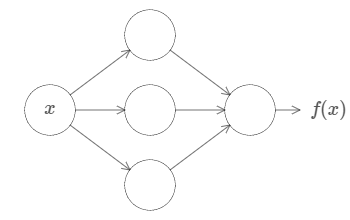
\includegraphics[width=0.43\linewidth]{figures/ch4/tikz400}
\end{center}
This result holds even if the function has many inputs, $f=f(x_1,\ldots,x_m)$, and many outputs. For instance, here's a network computing a function with $m=3$ inputs and $n=2$ outputs:
\begin{center}
	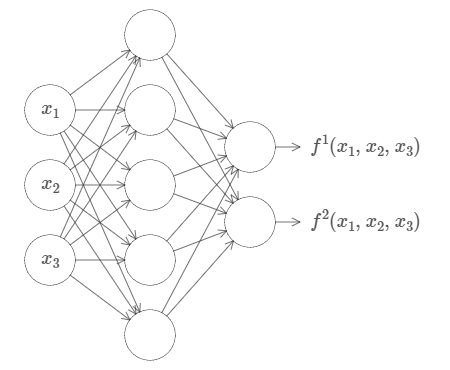
\includegraphics[width=0.45\linewidth]{figures/ch4/tikz401}
\end{center}
This result tells us that neural networks have a kind of \textit{universality}. No matter what function we want to compute, we know that there is a neural network which can do the job.

What's more, this universality theorem holds even if we restrict our networks to have just a single layer intermediate between the input and the output neurons -- a so-called single hidden layer. So even very simple network architectures can be extremely powerful.

The universality theorem is well known by people who use neural networks. But why it's true is not so widely understood. Most of the explanations available are quite technical. For instance, one of the original papers proving the result\footnote{\href{http://www.dartmouth.edu/~gvc/Cybenko_MCSS.pdf}{Approximation by superpositions of a sigmoidal function}, by George Cybenko (1989). The result was very much in the air at the time, and several groups proved closely related results. Cybenko's paper contains a useful discussion of much of that work. Another important early paper is [link]Multilayer feedforward networks are universal approximators, by Kurt Hornik, Maxwell Stinchcombe, and Halbert White (1989). This paper uses the Stone-Weierstrass theorem to arrive at similar results.} did so using the Hahn-Banach theorem, the Riesz Representation theorem, and some Fourier analysis. If you're a mathematician the argument is not difficult to follow, but it's not so easy for most people. That's a pity, since the underlying reasons for universality are simple and beautiful.

In this chapter I give a simple and mostly visual explanation of the universality theorem. We'll go step by step through the underlying ideas. You'll understand why it's true that neural networks can compute any function. You'll understand some of the limitations of the result. And you'll understand how the result relates to deep neural networks.

To follow the material in the chapter, you do not need to have read earlier chapters in this book. Instead, the chapter is structured to be enjoyable as a self-contained essay. Provided you have just a little basic familiarity with neural networks, you should be able to follow the explanation. I will, however, provide occasional links to earlier material, to help fill in any gaps in your knowledge.

Universality theorems are a commonplace in computer science, so much so that we sometimes forget how astonishing they are. But it's worth reminding ourselves: the ability to compute an arbitrary function is truly remarkable. Almost any process you can imagine can be thought of as function computation. Consider the problem of naming a piece of music based on a short sample of the piece. That can be thought of as computing a function. Or consider the problem of translating a Chinese text into English. Again, that can be thought of as computing a function\footnote{Actually, computing one of many functions, since there are often many acceptable translations of a given piece of text.}. Or consider the problem of taking an mp4 movie file and generating a description of the plot of the movie, and a discussion of the quality of the acting. Again, that can be thought of as a kind of function computation\footnote{Ditto the remark about translation and there being many possible functions..} Universality means that, in principle, neural networks can do all these things and many more.

Of course, just because we know a neural network exists that can (say) translate Chinese text into English, that doesn't mean we have good techniques for constructing or even recognizing such a network. This limitation applies also to traditional universality theorems for models such as Boolean circuits. But, as we've seen earlier in the book, neural networks have powerful algorithms for learning functions. That combination of learning algorithms + universality is an attractive mix. Up to now, the book has focused on the learning algorithms. In this chapter, we focus on universality, and what it means.


\section{Two caveats}
Before explaining why the universality theorem is true, I want to mention two caveats to the informal statement ``a neural network can compute any function''.

First, this doesn't mean that a network can be used to \textit{exactly} compute any function. Rather, we can get an \textit{approximation} that is as good as we want. By increasing the number of hidden neurons we can improve the approximation. For instance, earlier (see \ref{basic_network_precursor}) I illustrated a network computing some function $f(x)$ using three hidden neurons. For most functions only a low-quality approximation will be possible using three hidden neurons. By increasing the number of hidden neurons (say, to five) we can typically get a better approximation:
\begin{center}
	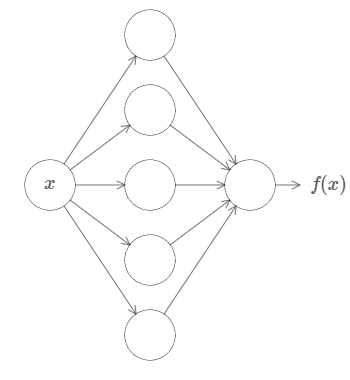
\includegraphics[width=0.43\linewidth]{figures/ch4/tikz402}
\end{center}
And we can do still better by further increasing the number of hidden neurons.

To make this statement more precise, suppose we're given a function $f(x)$ which we'd like to compute to within some desired accuracy $\epsilon>0$. The guarantee is that by using enough hidden neurons we can always find a neural network whose output $g(x)$ satisfies $|g(x)-f(x)|<\epsilon$, for all inputs $x$. In other words, the approximation will be good to within the desired accuracy for every possible input.

The second caveat is that the class of functions which can be approximated in the way described are the \textit{continuous} functions. If a function is discontinuous, i.e., makes sudden, sharp jumps, then it won't in general be possible to approximate using a neural net. This is not surprising, since our neural networks compute continuous functions of their input. However, even if the function we'd really like to compute is discontinuous, it's often the case that a continuous approximation is good enough. If that's so, then we can use a neural network. In practice, this is not usually an important limitation.

Summing up, a more precise statement of the universality theorem is that neural networks with a single hidden layer can be used to approximate any continuous function to any desired precision. In this chapter we'll actually prove a slightly weaker version of this result, using two hidden layers instead of one. In the problems I'll briefly outline how the explanation can, with a few tweaks, be adapted to give a proof which uses only a single hidden layer.

\section{Universality with one input and one output}
To understand why the universality theorem is true, let's start by understanding how to construct a neural network which approximates a function with just one input and one output:
\begin{center} 
	\begin{tikzpicture}
	\begin{axis}[title={$f(x)$},axis lines=middle,width=0.75\linewidth,height=0.5\linewidth,ymin=-0.05,ymax=1,scaled y ticks = false,y tick label style={/pgf/number format/fixed},xmin=-0.05,xmax=1.05,ticks=none]
	\addplot[blue,domain=0:1,samples=101]{0.2 + 0.4*x*x + 0.3*x*sin(15*deg(x)) + 0.05*cos(50*deg(x)) };
	\end{axis}
	\end{tikzpicture}
\end{center}
It turns out that this is the core of the problem of universality. Once we've understood this special case it's actually pretty easy to extend to functions with many inputs and many outputs.

To build insight into how to construct a network to compute $f$, let's start with a network containing just a single hidden layer, with two hidden neurons, and an output layer containing a single output neuron:
\begin{center}
	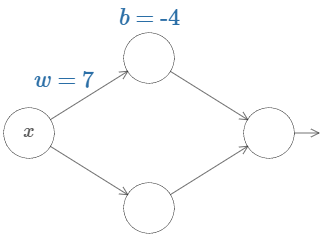
\includegraphics[width=0.45\linewidth]{figures/ch4/tikz403x}
\end{center}
To get a feel for how components in the network work, let's focus on the top hidden neuron. In the diagram below, click on the weight, $w$, and drag the mouse a little ways to the right to increase $w$. You can immediately see how the function computed by the top hidden neuron changes:
\begin{center}
\begin{tikzpicture}[declare function = {sigma(\x) = 1/(1+exp(-\x)); f(\x,\w,\b) = sigma(\w*\x+\b);}]
\pgfplotsset{every axis legend/.append style={at={(1.03,1)},anchor=north west}}

\begin{axis}[width=0.75\linewidth,height=0.45\linewidth,title={Output from neuron},axis x line=bottom,axis y line=left,xtick={0,1},ytick={0,1},xmax=1.05,ymax=1.05]
\addplot[blue!10!red,domain=0:1,samples=101]{f(x,7,-2)};
\addplot[blue!25!red,domain=0:1,samples=101]{f(x,7,-3)};
\addplot[blue!50!red,domain=0:1,samples=101]{f(x,7,-4)};
\addplot[blue!75!red,domain=0:1,samples=101]{f(x,7,-5)};
\addplot[blue!90!red,domain=0:1,samples=101]{f(x,7,-6)};
\addlegendentry{$w=7, b = -2$}
\addlegendentry{$w=7, b = -3$}
\addlegendentry{$w=7, b = -4$}
\addlegendentry{$w=7, b = -5$}
\addlegendentry{$w=7, b = -6$}
\end{axis}
\end{tikzpicture}
\end{center}
\begin{center}
	\begin{tikzpicture}[declare function = {sigma(\x) = 1/(1+exp(-\x)); f(\x,\w,\b) = sigma(\w*\x+\b);}]
	\pgfplotsset{every axis legend/.append style={at={(1.03,1)},anchor=north west}}

	\begin{axis}[width=0.75\linewidth,height=0.45\linewidth,title={Output from neuron},axis x line=bottom,axis y line=left,xtick={0,1},ytick={0,1},xmax=1.05,ymax=1.05]
	\addplot[blue!90!red,domain=0:1,samples=101]{f(x,9,-4)};
	\addplot[blue!75!red,domain=0:1,samples=101]{f(x,8,-4)};
	\addplot[blue!50!red,domain=0:1,samples=101]{f(x,7,-4)};
	\addplot[blue!25!red,domain=0:1,samples=101]{f(x,6,-4)};
	\addplot[blue!10!red,domain=0:1,samples=101]{f(x,5,-4)};
	\addlegendentry{$w=9, b = -4$}
	\addlegendentry{$w=8, b = -4$}
	\addlegendentry{$w=7, b = -4$}
	\addlegendentry{$w=6, b = -4$}
	\addlegendentry{$w=5, b = -4$}
	\end{axis}
	\end{tikzpicture}
\end{center}
As we learnt earlier in the book, what's being computed by the hidden neuron is $\sigma(wx+b)$, where $\sigma(z)\equiv1/(1+e^{-z})$ is the sigmoid function. Up to now, we've made frequent use of this algebraic form. But for the proof of universality we will obtain more insight by ignoring the algebra entirely, and instead manipulating and observing the shape shown in the graph. This won't just give us a better feel for what's going on, it will also give us a proof\footnote{Strictly speaking, the visual approach I'm taking isn't what's traditionally thought of as a proof. But I believe the visual approach gives more insight into why the result is true than a traditional proof. And, of course, that kind of insight is the real purpose behind a proof. Occasionally, there will be small gaps in the reasoning I present: places where I make a visual argument that is plausible, but not quite rigorous. If this bothers you, then consider it a challenge to fill in the missing steps. But don't lose sight of the real purpose: to understand why the universality theorem is true.} of universality that applies to activation functions other than the sigmoid function.
%
%To get started on this proof, try clicking on the bias, $b$, in the diagram above, and dragging to the right to increase it. You'll see that as the bias increases the graph moves to the left, but its shape doesn't change.
%
%Next, click and drag to the left in order to decrease the bias. You'll see that as the bias decreases the graph moves to the right, but, again, its shape doesn't change.
%
%Next, decrease the weight to around 2 or 3. You'll see that as you decrease the weight, the curve broadens out. You might need to change the bias as well, in order to keep the curve in-frame.
%
%Finally, increase the weight up past $w=100$. As you do, the curve gets steeper, until eventually it begins to look like a step function. Try to adjust the bias so the step occurs near $x=0.3$. The following short clip shows what your result should look like. Click on the play button to play (or replay) the video:
%\begin{lstlisting}
%ANIMATION
%\end{lstlisting}
We can simplify our analysis quite a bit by increasing the weight so much that the output really is a step function, to a very good approximation. Below I've plotted the output from the top hidden neuron when the weight is $w=999$. %Note that this plot is static, and you can't change parameters such as the weight.
%\begin{center}
%	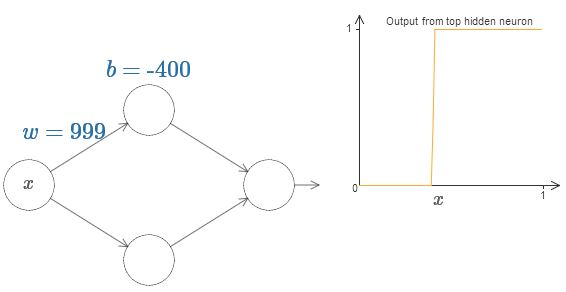
\includegraphics[width=0.7\linewidth]{figures/ch4/high_weight_function}
%\end{center}
\begin{center}
	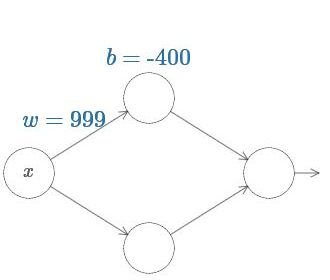
\includegraphics[width=0.35\linewidth]{figures/ch4/tikz403y}
	\begin{tikzpicture}[declare function = {sigma(\x,\w,\b) = 1/(1+exp(-\w*\x-\b));}]
		\begin{axis}[width=0.4\linewidth,height=0.4\linewidth,align=center,title={Output from top hidden neuron},axis x line=middle,axis y line=middle,xtick={0,1},ytick={0,1},xmax=1.15,ymax=1.15,ymin=-0.15,xlabel={$x$}]
		\addplot[blue!90!red,domain=0:1,samples=201]{sigma(x,999,-400)};
		\end{axis}
	\end{tikzpicture}
\end{center}
It's actually quite a bit easier to work with step functions than general sigmoid functions. The reason is that in the output layer we add up contributions from all the hidden neurons. It's easy to analyze the sum of a bunch of step functions, but rather more difficult to reason about what happens when you add up a bunch of sigmoid shaped curves. And so it makes things much easier to assume that our hidden neurons are outputting step functions. More concretely, we do this by fixing the weight $w$ to be some very large value, and then setting the position of the step by modifying the bias. Of course, treating the output as a step function is an approximation, but it's a very good approximation, and for now we'll treat it as exact. I'll come back later to discuss the impact of deviations from this approximation.

At what value of $x$ does the step occur? Put another way, how does the position of the step depend upon the weight and bias?

To answer this question, try modifying the weight and bias in the diagram above (you may need to scroll back a bit). Can you figure out how the position of the step depends on $w$ and $b$? With a little work you should be able to convince yourself that the position of the step is \textit{proportional} to $b$, and \textit{inversely proportional} to $w$.

In fact, the step is at position $s=-b/w$, as you can see by modifying the weight and bias in the following diagram:
\begin{center}
	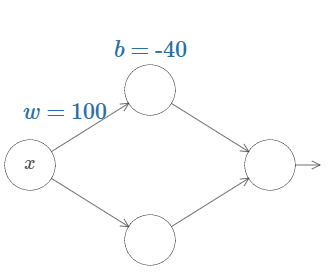
\includegraphics[width=0.35\linewidth]{figures/ch4/tikz404x}
	\begin{tikzpicture}[declare function = {sigma(\x,\w,\b) = 1/(1+exp(-\w*\x-\b));}]
		\begin{axis}[width=0.4\linewidth,height=0.4\linewidth,align=center,title={Output from top hidden neuron},axis x line=middle,axis y line=middle,xtick={0,0.4,1},xticklabels={0,$-b/w=0.4$,1},ytick={0,1},xmax=1.15,ymax=1.15,ymin=-0.15,xlabel={$x$}]
		\addplot[blue!90!red,domain=0:1,samples=201]{sigma(x,100,-40)};
		\end{axis}
	\end{tikzpicture}
\end{center}
It will greatly simplify our lives to describe hidden neurons using just a single parameter, $s$, which is the step position, $s=-b/w$. Try modifying s in the following diagram, in order to get used to the new parameterization:
\begin{center}
	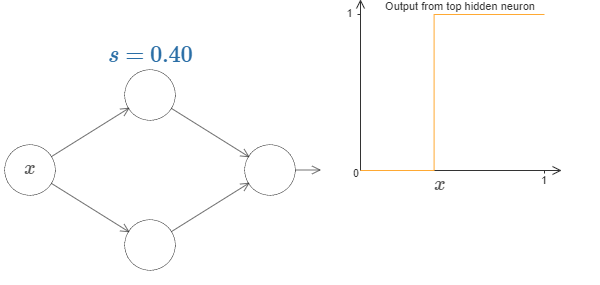
\includegraphics[width=0.35\linewidth]{figures/ch4/tikz405}
	\begin{tikzpicture}[declare function = {step(\x,\s)=0.5*(sign(\x-\s)+1);}]
		\begin{axis}[width=0.4\linewidth,height=0.4\linewidth,align=center,title={Output from top hidden neuron},axis x line=middle,axis y line=middle,xtick={0,0.4,1},xticklabels={0,$s$,1},ytick={0,1},xmax=1.15,ymax=1.15,ymin=-0.15,xlabel={$x$}]
		\addplot[blue!90!red,domain=0:1,samples=201]{step(x,0.4)};
		\end{axis}
	\end{tikzpicture}
\end{center}
%\begin{lstlisting}
%ANIMATIOIN
%\end{lstlisting}
As noted above, we've implicitly set the weight $w$ on the input to be some large value -- big enough that the step function is a very good approximation. We can easily convert a neuron parameterized in this way back into the conventional model, by choosing the bias $b=-ws$.

Up to now we've been focusing on the output from just the top hidden neuron. Let's take a look at the behavior of the entire network. In particular, we'll suppose the hidden neurons are computing step functions parameterized by step points $s_1$ (top neuron) and $s_2$ (bottom neuron). And they'll have respective output weights $w_1$ and $w_2$. Here's the network:
\begin{center}
	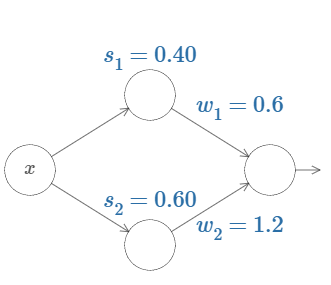
\includegraphics[width=0.35\linewidth]{figures/ch4/tikz407}
	\begin{tikzpicture}[declare function = {step(\x,\s,\h)=0.5*\h*(sign(\x-\s)+1);}]
		\begin{axis}[width=0.4\linewidth,height=0.4\linewidth,align=center,title={Weighted output from hidden layer},axis x line=middle,axis y line=middle,xtick={0,0.4,0.6,1},xticklabels={0,$s_1$,$s_2$,1},ytick={0,0.6,1,1.8},yticklabels={0,$w_1$,1,$w_1+w_2$},xmax=1.15,ymax=2.15,ymin=-0.15,xlabel={$x$}]
		\addplot[blue!90!red,domain=0:1,samples=201]{step(x,0.4,0.6)+step(x,0.6,1.2)};
		\end{axis}
	\end{tikzpicture}
\end{center}
%\begin{lstlisting}
%ANIMATIOIN
%\end{lstlisting}
What's being plotted on the right is the weighted output $w_1a_1+w_2a_2$ from the hidden layer. Here, $a_1$ and $a_2$ are the outputs from the top and bottom hidden neurons, respectively\footnote{Note, by the way, that the output from the whole network is $\sigma(w_1a_1+w_2a_2+b)$, where $b$ is the bias on the output neuron. Obviously, this isn't the same as the weighted output from the hidden layer, which is what we're plotting here. We're going to focus on the weighted output from the hidden layer right now, and only later will we think about how that relates to the output from the whole network.}. These outputs are denoted with as because they're often known as the neurons' activations.

Try increasing and decreasing the step point s1 of the top hidden neuron. Get a feel for how this changes the weighted output from the hidden layer. It's particularly worth understanding what happens when $s_1$ goes past $s_2$. You'll see that the graph changes shape when this happens, since we have moved from a situation where the top hidden neuron is the first to be activated to a situation where the bottom hidden neuron is the first to be activated.

Similarly, try manipulating the step point $s_2$ of the bottom hidden neuron, and get a feel for how this changes the combined output from the hidden neurons.

Try increasing and decreasing each of the output weights. Notice how this rescales the contribution from the respective hidden neurons. What happens when one of the weights is zero?

Finally, try setting $w_1$ to be 0.8 and $w_2$ to be -0.8. You get a ``bump'' function, which starts at point $s_1$, ends at point $s_2$, and has height 0.8. For instance, the weighted output might look like this:
\begin{center}
	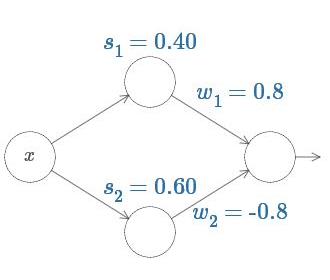
\includegraphics[width=0.35\linewidth]{figures/ch4/tikz408}
	\begin{tikzpicture}[declare function = {step(\x,\s,\h)=0.5*\h*(sign(\x-\s)+1);}]
		\begin{axis}[width=0.4\linewidth,height=0.4\linewidth,align=center,title={Weighted output from hidden layer},axis x line=middle,axis y line=middle,xtick={0,0.4,0.6,1},xticklabels={0,$s_1$,$s_2$,1},ytick={0,0.8,1},yticklabels={0,$w_1=-w_2$,1},xmax=1.15,ymax=2.15,ymin=-0.15,xlabel={$x$}]
		\addplot[blue!90!red,domain=0:1,samples=201]{step(x,0.4,0.8)+step(x,0.6,-0.8)};
		\end{axis}
	\end{tikzpicture}
\end{center}
Of course, we can rescale the bump to have any height at all. Let's use a single parameter, $h$, to denote the height. To reduce clutter I'll also remove the ``$s_1=\ldots$'' and ``$w_1=\ldots$'' notations.
\begin{center}
	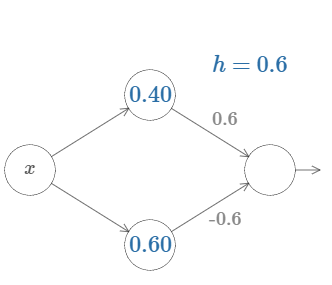
\includegraphics[width=0.35\linewidth]{figures/ch4/tikz406}
	\begin{tikzpicture}[declare function = {bump(\x,\s,\t,\h)=0.5*\h*(sign(\x-\s)-sign(\x-\t));}]
	\begin{axis}[width=0.4\linewidth,height=0.4\linewidth,align=center,title={Weighted output from hidden layer},axis x line=middle,axis y line=middle,xtick={0,0.4,0.6,1},xticklabels={0,$s_1$,$s_2$,1},ytick={-1,0,0.6,1},yticklabels={$-1$,0,$h$,1},xmax=1.25,ymax=1.25,ymin=-1.25,xlabel={$x$}]
	\addplot[blue!90!red,domain=0:1,samples=201]{bump(x,0.4,0.6,0.6};
	\end{axis}
	\end{tikzpicture}
\end{center}
Try changing the value of $h$ up and down, to see how the height of the bump changes. Try changing the height so it's negative, and observe what happens. And try changing the step points to see how that changes the shape of the bump.

You'll notice, by the way, that we're using our neurons in a way that can be thought of not just in graphical terms, but in more conventional programming terms, as a kind of \texttt{if-then-else} statement, e.g.:
\begin{lstlisting}
if input >= step point:
	add 1 to the weighted output
else:
	add 0 to the weighted output
\end{lstlisting}
For the most part I'm going to stick with the graphical point of view. But in what follows you may sometimes find it helpful to switch points of view, and think about things in terms of \texttt{if-then-else}.

We can use our bump-making trick to get two bumps, by gluing two pairs of hidden neurons together into the same network:
\begin{center}
	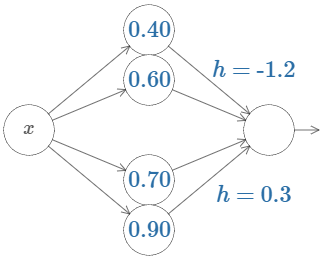
\includegraphics[width=0.35\linewidth]{figures/ch4/tikz421}
	\begin{tikzpicture}[declare function = {step(\x,\s,\t)=0.5*(sign(\x-\s)-sign(\x-\t));twobumps(\x,\s,\t,\h,\ss,\tt,\hh) = \h*step(\x,\s,\t)+\hh*step(\x,\ss,\tt); }]
	\begin{axis}[width=0.4\linewidth,height=0.4\linewidth,align=center,title={Weighted output from hidden layer},axis x line=bottom,axis y line=left,xtick={0,0.4,0.6,0.7,0.9,1},xticklabels={0,$s_1^1$,$s_2^1$,$s_1^2$,$s_2^2$,1},ytick={-1.2,-1,0,0.3,1},yticklabels={$h_1$,$-1$,0,$h_2$,1},xmax=1.15,ymax=1.25,ymin=-1.25]
	\addplot[blue!90!red,domain=0:1,samples=201]{twobumps(x,0.4,0.6,-1.2,0.7,0.9,0.3};
	\end{axis}
	\end{tikzpicture}
\end{center}
I've suppressed the weights here, simply writing the $h$ values for each pair of hidden neurons. Try increasing and decreasing both h values, and observe how it changes the graph. Move the bumps around by changing the step points.

More generally, we can use this idea to get as many peaks as we want, of any height. In particular, we can divide the interval [0,1] up into a large number, $N$, of subintervals, and use $N$ pairs of hidden neurons to set up peaks of any desired height. Let's see how this works for $N=5$. That's quite a few neurons, so I'm going to pack things in a bit. Apologies for the complexity of the diagram: I could hide the complexity by abstracting away further, but I think it's worth putting up with a little complexity, for the sake of getting a more concrete feel for how these networks work.
\begin{center}
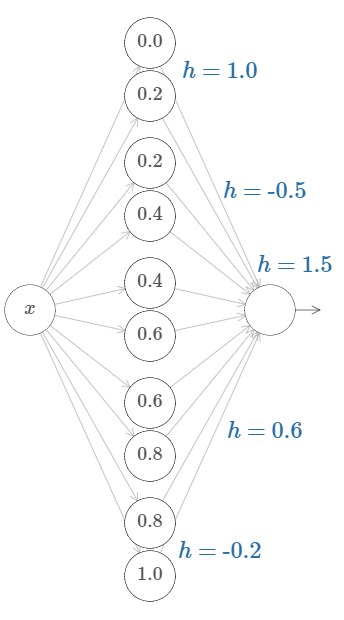
\includegraphics[height=0.65\linewidth]{./figures/ch4/tikz438}
\begin{tikzpicture}[declare function = {step(\x,\s,\t)=0.5*(sign(\x-\s)-sign(\x-\t));}]
\begin{axis}[width=0.42\linewidth,height=0.65\linewidth,align=center,title={Weighted output},axis x line=middle,axis y line=left,xtick={0,1},ytick={-1,0,1},xmax=1.15,ymax=2.2,ymin=-1.5]
	\addplot[blue!90!red,domain=0:1.05,samples=201]{step(x,0,0.2)};
	\addplot[blue!90!red,domain=0:1.05,samples=201]{-0.5*step(x,0.2,0.4)};
	\addplot[blue!90!red,domain=0:1.05,samples=201]{+1.5*step(x,0.4,0.6)};
	\addplot[blue!90!red,domain=0:1.05,samples=201]{+0.6*step(x,0.6,0.8)};
	\addplot[blue!90!red,domain=0:1.05,samples=201]{-0.2*step(x,0.8,1.0)};
	\end{axis}
\end{tikzpicture}	
\end{center}
You can see that there are five pairs of hidden neurons. The step points for the respective pairs of neurons are 0,1/5, then 1/5,2/5, and so on, out to 4/5,5/5. These values are fixed -- they make it so we get five evenly spaced bumps on the graph.

Each pair of neurons has a value of $h$ associated to it. Remember, the connections output from the neurons have weights $h$ and $-h$ (not marked). Click on one of the $h$ values, and drag the mouse to the right or left to change the value. As you do so, watch the function change. By changing the output weights we're actually \textit{designing} the function!

Contrariwise, try clicking on the graph, and dragging up or down to change the height of any of the bump functions. As you change the heights, you can see the corresponding change in $h$ values. And, although it's not shown, there is also a change in the corresponding output weights, which are $+h$ and $-h$.

In other words, we can directly manipulate the function appearing in the graph on the right, and see that reflected in the h values on the left. A fun thing to do is to hold the mouse button down and drag the mouse from one side of the graph to the other. As you do this you draw out a function, and get to watch the parameters in the neural network adapt.

Time for a challenge.

Let's think back to the function I plotted at the beginning of the chapter:
\begin{center} 
	\begin{tikzpicture}
	\begin{axis}[title={$f(x)$},axis lines=middle,width=0.6\linewidth,height=0.5\linewidth,ymin=-0.05,ymax=1,scaled y ticks = false,y tick label style={/pgf/number format/fixed},xmin=-0.05,xmax=1.05,ticks=none]
	\addplot[blue,domain=0:1,samples=101]{0.2 + 0.4*x*x + 0.3*x*sin(15*deg(x)) + 0.05*cos(50*deg(x)) };
	\end{axis}
	\end{tikzpicture}
\end{center}
I didn't say it at the time, but what I plotted is actually the function
\begin{equation}
f(x)=0.2+0.4x^2+0.3x\sin(15x)+0.05\cos(50x),\label{eq:113}
\end{equation}
plotted over $x$ from 0 to 1, and with the $y$ axis taking values from 0 to 1.

That's obviously not a trivial function.

You're going to figure out how to compute it using a neural network.

In our networks above we've been analyzing the weighted combination $\sum_jw_ja_j$ output from the hidden neurons. We now know how to get a lot of control over this quantity. But, as I noted earlier, this quantity is not what's output from the network. What's output from the network is $\sigma(\sum_jw_ja_j+b)$ where $b$ is the bias on the output neuron. Is there some way we can achieve control over the actual output from the network?

The solution is to design a neural network whose hidden layer has a weighted output given by $\sigma^{-1} \circ f(x)$, where $\sigma^{-1}$ is just the inverse of the $\sigma$ function. That is, we want the weighted output from the hidden layer to be:
\begin{center} 
	\begin{tikzpicture}
	\begin{axis}[axis lines=middle,width=0.6\linewidth,height=0.5\linewidth,ymin=-2.05,ymax=2.25,scaled y ticks = false,y tick label style={/pgf/number format/fixed},xmin=-0.05,xmax=1.05, xtick={0,1}]
	\addplot[blue,domain=0:1,samples=101]{4*(-0.3 + 0.4*x*x + 0.3*x*sin(15*deg(x)) + 0.05*cos(50*deg(x))) };
	\node[anchor=north,align=center] at (axis cs: 0.5,2) {$\sigma^{-1}\circ f(x)$};
	\end{axis}
	\end{tikzpicture}
\end{center}
If we can do this, then the output from the network as a whole will be a good approximation to $f(x)$\footnote{Note that I have set the bias on the output neuron to 0.}.

Your challenge, then, is to design a neural network to approximate the goal function shown just above. To learn as much as possible, I want you to solve the problem twice. The first time, please click on the graph, directly adjusting the heights of the different bump functions. You should find it fairly easy to get a good match to the goal function. How well you're doing is measured by the average deviation between the goal function and the function the network is actually computing. Your challenge is to drive the average deviation as low as possible. You complete the challenge when you drive the average deviation to 0.40 or below\footnote{This paragraph refers to interactive element, available online. The graph shows the final result of manual minimization of average deviation. }

%Once you've done that, click on ``Reset'' to randomly re-initialize the bumps. The second time you solve the problem, resist the urge to click on the graph. Instead, modify the h values on the left-hand side, and again attempt to drive the average deviation to 0.40 or below.
\begin{center} 
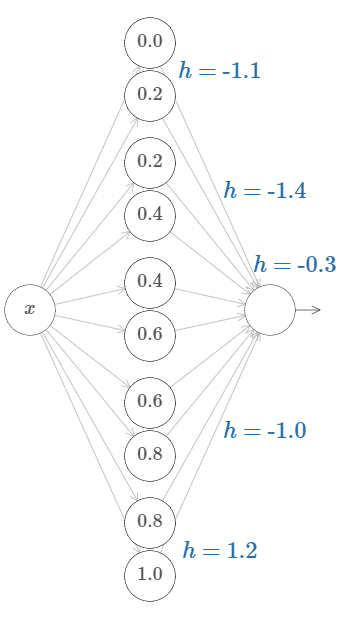
\includegraphics[height=0.65\textwidth]{./figures/ch4/tikz439}
\begin{tikzpicture}[declare function = {step(\x,\s,\t)=0.5*(sign(\x-\s)-sign(\x-\t));}]
	\begin{axis}[axis lines=middle,width=0.6\textwidth,height=0.65\textwidth,ymin=-2.05,ymax=2.25,scaled y ticks = false,y tick label style={/pgf/number format/fixed},xmin=-0.05,xmax=1.05, xtick={0,1}]
		\addplot[blue,domain=0:1,samples=101]{4*(-0.3 + 0.4*x*x + 0.3*x*sin(15*deg(x)) + 0.05*cos(50*deg(x))) };
		\addplot[red!50!black,domain=0:1.05,samples=201]{-1.1*step(x,0,0.2)};
		\addplot[red!50!black,domain=0:1.05,samples=201]{-1.4*step(x,0.2,0.4)};
		\addplot[red!50!black,domain=0:1.05,samples=201]{-0.3*step(x,0.4,0.6)};
		\addplot[red!50!black,domain=0:1.05,samples=201]{-1*step(x,0.6,0.8)};
		\addplot[red!50!black,domain=0:1.05,samples=201]{+1.2*step(x,0.8,1.0)};
		\node[anchor=north,align=center] at (axis cs: 0.5,2) {Weighted output\\$\sigma = 0.38$};
	\end{axis}
\end{tikzpicture}
\end{center}
You've now figured out all the elements necessary for the network to approximately compute the function $f(x)$! It's only a coarse approximation, but we could easily do much better, merely by increasing the number of pairs of hidden neurons, allowing more bumps.

In particular, it's easy to convert all the data we have found back into the standard parameterization used for neural networks. Let me just recap quickly how that works.

The first layer of weights all have some large, constant value, say $w=1000$.

The biases on the hidden neurons are just $b=-ws$. So, for instance, for the second hidden neuron $s=0.2$ becomes $b=-1000\times0.2=-200$.

The final layer of weights are determined by the $h$ values. So, for instance, the value you've chosen above for the first $h$, $h= -0.6$, means that the output weights from the top two hidden neurons are $-0.6$ and 0.6, respectively. And so on, for the entire layer of output weights.

Finally, the bias on the output neuron is 0.

That's everything: we now have a complete description of a neural network which does a pretty good job computing our original goal function. And we understand how to improve the quality of the approximation by improving the number of hidden neurons.

What's more, there was nothing special about our original goal function, $f(x)=0.2+0.4x^2+0.3\sin(15x)+0.05\cos(50x)$. We could have used this procedure for any continuous function from [0,1] to [0,1]. In essence, we're using our single-layer neural networks to build a lookup table for the function. And we'll be able to build on this idea to provide a general proof of universality.

\section{Many input variables}
Let's extend our results to the case of many input variables. This sounds complicated, but all the ideas we need can be understood in the case of just two inputs. So let's address the two-input case.

We'll start by considering what happens when we have two inputs to a neuron:
\begin{center}
	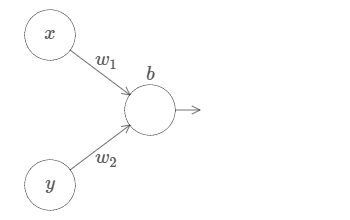
\includegraphics[width=0.4\linewidth]{figures/ch4/tikz411}
\end{center}
Here, we have inputs $x$ and $y$, with corresponding weights $w_1$ and $w_2$, and a bias $b$ on the neuron. Let's set the weight $w_2$ to 0, and then play around with the first weight, $w_1$, and the bias, $b$, to see how they affect the output from the neuron:
\begin{center}
	\begin{tikzpicture}[scale=0.8]
		\begin{axis}[colormap={justred}{rgb255=(255,127,127);rgb255=(127,31,31)}, grid=major,width=5cm,height=6cm,view={-15}{10},xlabel={$x$},ylabel={$y$},zlabel={Output},title={$w_1=8,b=-8$},zmin=0,zmax=1,xtick={0,1},ytick={0,1},zmajorticks=false]
			\addplot3[surf, domain=0:1,samples=26,shader=faceted]{1/(1+exp(-(8*x-8)))};
			\end{axis}
	\end{tikzpicture}
	\begin{tikzpicture}[scale=0.8]
		\begin{axis}[colormap={justred}{rgb255=(255,127,127);rgb255=(127,31,31)},grid=major,width=5cm,height=6cm,view={-15}{10},xlabel={$x$},ylabel={$y$},zlabel={Output},title={$w_1=8,b=-5$},zmin=0,zmax=1,xtick={0,1},ytick={0,1},zmajorticks=false]
			\addplot3[surf, domain=0:1,samples=26,shader=faceted]{1/(1+exp(-(8*x-5)))};
		\end{axis}
	\end{tikzpicture}
	\begin{tikzpicture}[scale=0.8]
		\begin{axis}[colormap={justred}{rgb255=(255,127,127);rgb255=(127,31,31)},grid=major,width=5cm,height=6cm,view={-15}{10},xlabel={$x$},ylabel={$y$},zlabel={Output},title={$w_1=8,b=-2$},zmin=0,zmax=1,xtick={0,1},ytick={0,1},zmajorticks=false]
			\addplot3[surf, domain=0:1,samples=26,shader=faceted]{1/(1+exp(-(8*x-2)))};
		\end{axis}
	\end{tikzpicture}
\end{center}

\begin{center}
	\begin{tikzpicture}[scale=0.8]
		\begin{axis}[colormap={justred}{rgb255=(255,127,127);rgb255=(127,31,31)},grid=major,width=5cm,height=6cm,view={-15}{10},xlabel={$x$},ylabel={$y$},zlabel={Output},title={$w_1=11,b=-5$},zmin=0,zmax=1,xtick={0,1},ytick={0,1},zmajorticks=false]
			\addplot3[surf, domain=0:1,samples=26,shader=faceted]{1/(1+exp(-(11*x-5)))};
			\end{axis}
	\end{tikzpicture}
	\begin{tikzpicture}[scale=0.8]
		\begin{axis}[colormap={justred}{rgb255=(255,127,127);rgb255=(127,31,31)},grid=major,width=5cm,height=6cm,view={-15}{10},xlabel={$x$},ylabel={$y$},zlabel={Output},title={$w_1=8,b=-5$},zmin=0,zmax=1,xtick={0,1},ytick={0,1},zmajorticks=false]
			\addplot3[surf, domain=0:1,samples=26,shader=faceted]{1/(1+exp(-(8*x-5)))};
		\end{axis}
	\end{tikzpicture}
	\begin{tikzpicture}[scale=0.8]
		\begin{axis}[colormap={justred}{rgb255=(255,127,127);rgb255=(127,31,31)},grid=major,width=5cm,height=6cm,view={-15}{10},xlabel={$x$},ylabel={$y$},zlabel={Output},title={$w_1=5,b=-5$},zmin=0,zmax=1,xtick={0,1},ytick={0,1},zmajorticks=false]
			\addplot3[surf, domain=0:1,samples=26,shader=faceted]{1/(1+exp(-(5*x-5)))};
		\end{axis}
	\end{tikzpicture}
\end{center}
%
%x=1y=1Output
%
As you can see, with $w_2=0$ the input $y$ makes no difference to the output from the neuron. It's as though $x$ is the only input.

Given this, what do you think happens when we increase the weight $w_1$ to $w_1=100$, with $w_2$ remaining 0? If you don't immediately see the answer, ponder the question for a bit, and see if you can figure out what happens. Then try it out and see if you're right. I've shown what happens in the following movie:


Just as in our earlier discussion, as the input weight gets larger the output approaches a step function. The difference is that now the step function is in three dimensions. Also as before, we can move the location of the step point around by modifying the bias. The actual location of the step point is $s_x\equiv-b/w_1$.

Let's redo the above using the position of the step as the parameter:
\begin{center}
	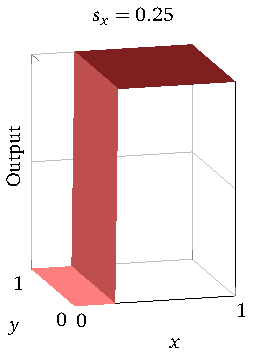
\includegraphics[width=0.32\linewidth]{./figures/ch4/3d/stepx1}
	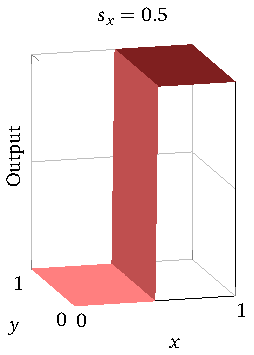
\includegraphics[width=0.32\linewidth]{./figures/ch4/3d/stepx2}
	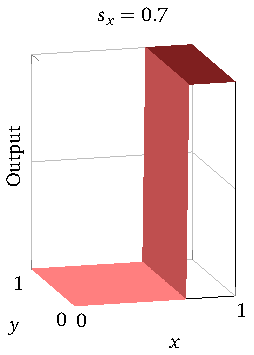
\includegraphics[width=0.32\linewidth]{./figures/ch4/3d/stepx3}
%	\begin{tikzpicture}[scale=0.8]
%		\begin{axis}[colormap={justred}{rgb255=(255,127,127);rgb255=(127,31,31)},grid=major,width=5cm,height=0.45\linewidth,view={-15}{10},xlabel={$x$},ylabel={$y$},zlabel={Output},title={$s_x=0.25$},zmin=0,zmax=1,xtick={0,1},ytick={0,1},zmajorticks=false]
%			\addplot3[surf, domain=0:1,samples=26,shader=faceted]{1/(1+exp(-1000*(x-0.25)))};
%			\end{axis}
%	\end{tikzpicture}
%	\begin{tikzpicture}[scale=0.8]
%		\begin{axis}[colormap={justred}{rgb255=(255,127,127);rgb255=(127,31,31)},grid=major,width=5cm,height=0.45\linewidth,view={-15}{10},xlabel={$x$},ylabel={$y$},title={$s_x=0.5$},zmin=0,zmax=1,xtick={0,1},ytick={0,1},zmajorticks=false]
%			\addplot3[surf, domain=0:1,samples=26,shader=faceted]{1/(1+exp(-1000*(x-0.5)))};
%		\end{axis}
%	\end{tikzpicture}
%	\begin{tikzpicture}[scale=0.8]
%		\begin{axis}[colormap={justred}{rgb255=(255,127,127);rgb255=(127,31,31)},grid=major,width=5cm,height=0.45\linewidth,view={-15}{10},xlabel={$x$},ylabel={$y$},title={$s_x=0.7$},zmin=0,zmax=1,xtick={0,1},ytick={0,1},zmajorticks=false]
%			\addplot3[surf, domain=0:1,samples=26,shader=faceted]{1/(1+exp(-1000*(x-0.7)))};
%		\end{axis}
%	\end{tikzpicture}
\end{center}
Here, we assume the weight on the $x$ input has some large value -- I've used $w_1=1000$ -- and the weight $w_2=0$. The number on the neuron is the step point, and the little $x$ above the number reminds us that the step is in the x direction. Of course, it's also possible to get a step function in the $y$ direction, by making the weight on the $y$ input very large (say, $w_2=1000$), and the weight on the $x$ equal to 0, i.e., $w_1=0$:
\begin{center}
%	\begin{tikzpicture}[scale=0.8]
%		\begin{axis}[colormap={justred}{rgb255=(255,127,127);rgb255=(127,31,31)},grid=major,width=5cm,height=0.45\linewidth,view={-15}{10},xlabel={$x$},ylabel={$y$},zlabel={Output},title={$s_y=0.25$},zmin=0,zmax=1,xtick={0,1},ytick={0,1},zmajorticks=false]
%			\addplot3[surf, domain=0:1,samples=26,shader=faceted]{1/(1+exp(-1000*(y-0.25)))};
%			\end{axis}
%	\end{tikzpicture}
%	\begin{tikzpicture}[scale=0.8]
%		\begin{axis}[colormap={justred}{rgb255=(255,127,127);rgb255=(127,31,31)},grid=major,width=5cm,height=0.45\linewidth,view={-15}{10},xlabel={$x$},ylabel={$y$},title={$s_y=0.5$},zmin=0,zmax=1,xtick={0,1},ytick={0,1},zmajorticks=false]
%			\addplot3[surf, domain=0:1,samples=26,shader=faceted]{1/(1+exp(-1000*(y-0.5)))};
%		\end{axis}
%	\end{tikzpicture}
%	\begin{tikzpicture}[scale=0.8]
%		\begin{axis}[colormap={justred}{rgb255=(255,127,127);rgb255=(127,31,31)},grid=major,width=5cm,height=0.45\linewidth,view={-15}{10},xlabel={$x$},ylabel={$y$},title={$s_y=0.7$},zmin=0,zmax=1,xtick={0,1},ytick={0,1},zmajorticks=false]
%			\addplot3[surf, domain=0:1,samples=26,shader=faceted]{1/(1+exp(-1000*(y-0.7)))};
%		\end{axis}
%	\end{tikzpicture}
	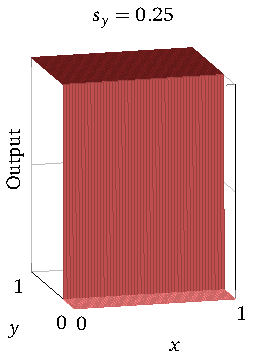
\includegraphics[width=0.32\linewidth]{./figures/ch4/3d/stepy1}
	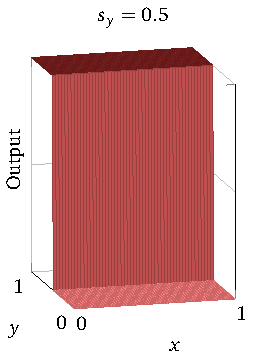
\includegraphics[width=0.32\linewidth]{./figures/ch4/3d/stepy2}
	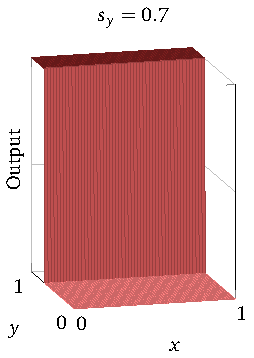
\includegraphics[width=0.32\linewidth]{./figures/ch4/3d/stepy3}
\end{center}
The number on the neuron is again the step point, and in this case the little $y$ above the number reminds us that the step is in the $y$ direction. I could have explicitly marked the weights on the $x$ and $y$ inputs, but decided not to, since it would make the diagram rather cluttered. But do keep in mind that the little $y$ marker implicitly tells us that the $y$ weight is large, and the $x$ weight is 0.

We can use the step functions we've just constructed to compute a three-dimensional bump function. To do this, we use two neurons, each computing a step function in the $x$ direction. Then we combine those step functions with weight $h$ and $-h$, respectively, where $h$ is the desired height of the bump. It's all illustrated in the following diagram:
\begin{center}
%	\begin{tikzpicture}[scale=0.8]
%		\begin{axis}[colormap={justred}{rgb255=(255,127,127);rgb255=(127,31,31)},grid=major,width=5cm,height=0.45\linewidth,view={-15}{10},xlabel={$x$},ylabel={$y$},zlabel={Output},title={$s^1_x=0.25,s^2_x=0.75, h=1$},zmin=0,zmax=1,xtick={0,1},ytick={0,1},zmajorticks=false]
%			\addplot3[surf, domain=0:1,samples=26,shader=faceted]{1/(1+exp(-100*(x-0.25)))-1/(1+exp(-100*(x-0.75)))};
%			\end{axis}
%	\end{tikzpicture}
%	\begin{tikzpicture}[scale=0.8]
%		\begin{axis}[colormap={justred}{rgb255=(255,127,127);rgb255=(127,31,31)},grid=major,width=5cm,height=0.45\linewidth,view={-15}{10},xlabel={$x$},ylabel={$y$},title={$s^1_x=0.25,s^2_x=0.75, h=0.75$},zmin=0,zmax=1,xtick={0,1},ytick={0,1},zmajorticks=false]
%			\addplot3[surf, domain=0:1,samples=26,shader=faceted]{0.75/(1+exp(-100*(x-0.25)))-0.75/(1+exp(-100*(x-0.75)))};
%		\end{axis}
%	\end{tikzpicture}
%%		\begin{axis}[colormap={justred}{rgb255=(255,127,127);rgb255=(127,31,31)},grid=major,width=5cm,height=0.45\linewidth,view={-15}{10},xlabel={$x$},ylabel={$y$},title={$s^1_x=0.5,s^2_x=0.75, h=1$},zmin=0,zmax=1,xtick={0,1},ytick={0,1},zmajorticks=false]
%			\addplot3[surf, domain=0:1,samples=26,shader=faceted]{1/(1+exp(-100*(x-0.5)))-1/(1+exp(-100*(x-0.75)))};
%		\end{axis}
%	\end{tikzpicture}
	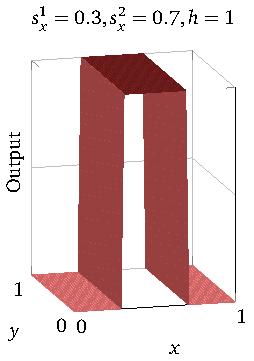
\includegraphics[width=0.32\linewidth]{./figures/ch4/3d/bumpx1}
	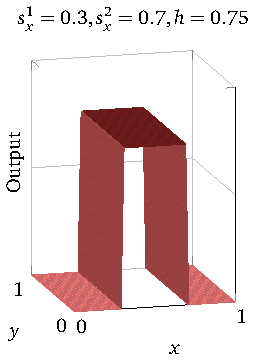
\includegraphics[width=0.32\linewidth]{./figures/ch4/3d/bumpx2}
	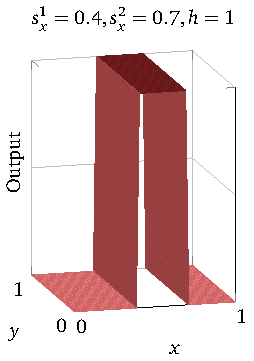
\includegraphics[width=0.32\linewidth]{./figures/ch4/3d/bumpx3}
\end{center}
%
%x=1y=1Weighted output from hidden layer
%
Try changing the value of the height, h. Observe how it relates to the weights in the network. And see how it changes the height of the bump function on the right.

Also, try changing the step point 0.30 associated to the top hidden neuron. Witness how it changes the shape of the bump. What happens when you move it past the step point 0.70 associated to the bottom hidden neuron?

We've figured out how to make a bump function in the $x$ direction. Of course, we can easily make a bump function in the $y$ direction, by using two step functions in the $y$ direction. Recall that we do this by making the weight large on the $y$ input, and the weight 0 on the $x$ input. Here's the result:
\begin{center}
	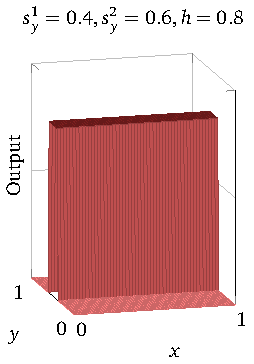
\includegraphics[width=0.32\linewidth]{./figures/ch4/3d/bumpy1}
	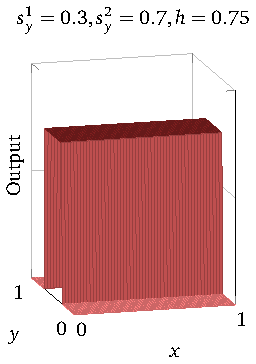
\includegraphics[width=0.32\linewidth]{./figures/ch4/3d/bumpy2}
	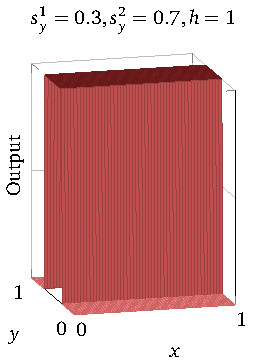
\includegraphics[width=0.32\linewidth]{./figures/ch4/3d/bumpy3}
%	\begin{tikzpicture}[scale=0.8]
%		\begin{axis}[colormap={justred}{rgb255=(255,127,127);rgb255=(127,31,31)},grid=major,width=5cm,height=0.45\linewidth,view={-15}{10},xlabel={$x$},ylabel={$y$},zlabel={Output},title={$s^1_y=0.25,s^2_y=0.75, h=1$},zmin=0,zmax=1,xtick={0,1},ytick={0,1},zmajorticks=false]
%			\addplot3[surf, domain=0:1,samples=26,shader=faceted]{1/(1+exp(-100*(y-0.25)))-1/(1+exp(-100*(y-0.75)))};
%			\end{axis}
%	\end{tikzpicture}
%	\begin{tikzpicture}[scale=0.8]
%		\begin{axis}[colormap={justred}{rgb255=(255,127,127);rgb255=(127,31,31)},grid=major,width=5cm,height=0.45\linewidth,view={-15}{10},xlabel={$x$},ylabel={$y$},title={$s^1_y=0.25,s^2_y=0.75, h=0.75$},zmin=0,zmax=1,xtick={0,1},ytick={0,1},zmajorticks=false]
%			\addplot3[surf, domain=0:1,samples=26,shader=faceted]{0.75/(1+exp(-100*(y-0.25)))-0.75/(1+exp(-100*(y-0.75)))};
%		\end{axis}
%	\end{tikzpicture}
%	\begin{tikzpicture}[scale=0.8]
%		\begin{axis}[colormap={justred}{rgb255=(255,127,127);rgb255=(127,31,31)},grid=major,width=5cm,height=0.45\linewidth,view={-15}{10},xlabel={$x$},ylabel={$y$},title={$s^1_y=0.25,s^2_y=0.45, h=0.8$},zmin=0,zmax=1,xtick={0,1},ytick={0,1},zmajorticks=false]
%			\addplot3[surf, domain=0:1,samples=26,shader=faceted]{0.8/(1+exp(-100*(y-0.25)))-0.8/(1+exp(-100*(y-0.45)))};
%		\end{axis}
%	\end{tikzpicture}
\end{center}
%
%x=1y=1Weighted output from hidden layer
%
This looks nearly identical to the earlier network! The only thing explicitly shown as changing is that there's now little $y$ markers on our hidden neurons. That reminds us that they're producing y step functions, not x step functions, and so the weight is very large on the y input, and zero on the x input, not vice versa. As before, I decided not to show this explicitly, in order to avoid clutter.
%
Let's consider what happens when we add up two bump functions, one in the $x$ direction, the other in the $y$ direction, both of height $h$:
\begin{center}
%	\begin{tikzpicture}[scale=0.8]
%		\begin{axis}[colormap={justred}{rgb255=(255,127,127);rgb255=(127,31,31)},grid=major,width=5cm,height=0.45\linewidth,view={-15}{10},xlabel={$x$},ylabel={$y$},zlabel={Output},title={$s^1_x=0.4,s^2_x=0.6,s^1_y=0.3,s^2_y=0.7, h=1$},zmin=0,zmax=1,xtick={0,1},ytick={0,1},zmajorticks=false]
%			\addplot3[surf, domain=0:1,samples=26,shader=faceted]{0.5/(1+exp(-100*(y-0.3)))-0.5/(1+exp(-100*(y-0.7)))+0.5/(1+exp(-100*(x-0.4)))-0.5/(1+exp(-100*(x-0.6)))};
%			\end{axis}
%	\end{tikzpicture}
%	\begin{tikzpicture}[scale=0.8]
%		\begin{axis}[colormap={justred}{rgb255=(255,127,127);rgb255=(127,31,31)},grid=major,width=5cm,height=0.45\linewidth,view={-15}{10},xlabel={$x$},ylabel={$y$},title={$s^1_x=0.4,s^2_x=0.6,s^1_y=0.3,s^2_y=0.7, h=0.5$},zmin=0,zmax=1,xtick={0,1},ytick={0,1},zmajorticks=false]
%			\addplot3[surf, domain=0:1,samples=26,shader=faceted]{0.25/(1+exp(-100*(y-0.3)))-0.25/(1+exp(-100*(y-0.7)))+0.25/(1+exp(-100*(x-0.4)))-0.25/(1+exp(-100*(x-0.6)))};
%		\end{axis}
%	\end{tikzpicture}
	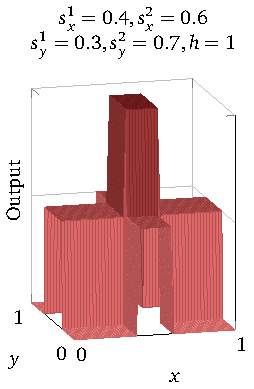
\includegraphics[width=0.32\linewidth]{./figures/ch4/3d/bumpxy1}
	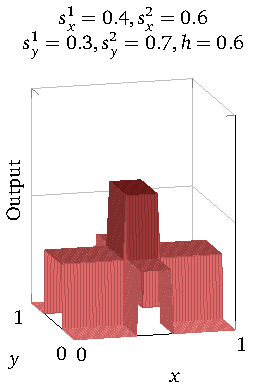
\includegraphics[width=0.32\linewidth]{./figures/ch4/3d/bumpxy2}
\end{center}
To simplify the diagram I've dropped the connections with zero weight. For now, I've left in the little x and y markers on the hidden neurons, to remind you in what directions the bump functions are being computed. We'll drop even those markers later, since they're implied by the input variable.
%
Try varying the parameter $h$. As you can see, this causes the output weights to change, and also the heights of both the x and y bump functions.
%
What we've built looks a little like a \textit{tower} function:
\begin{center}
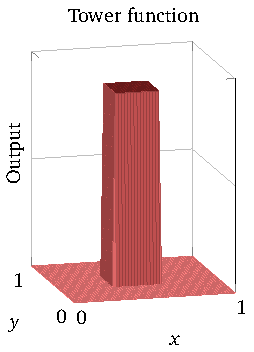
\includegraphics[width=0.32\linewidth]{./figures/ch4/3d/towerfunction}%	\begin{tikzpicture}[scale=0.8]
%			\begin{axis}[colormap={justred}{rgb255=(255,127,127);rgb255=(127,31,31)},grid=major,width=5cm,height=0.45\linewidth,view={-15}{10},xlabel={$x$},ylabel={$y$},zlabel={Output},title={Tower function},zmin=0,zmax=1,xtick={0,1},ytick={0,1},zmajorticks=false]
%				\addplot3[surf, domain=0:1,samples=26,shader=faceted]{(1/(1+exp(-100*(y-0.4)))-1/(1+exp(-100*(y-0.6))))*(1/(1+exp(-100*(x-0.4)))-1/(1+exp(-100*(x-0.6))))};
%				\end{axis}
%		\end{tikzpicture}
\end{center}
%
%x=1y=1Tower function
If we could build such tower functions, then we could use them to approximate arbitrary functions, just by adding up many towers of different heights, and in different locations:
\begin{center}
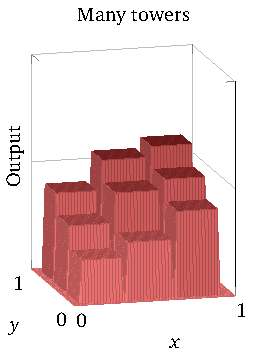
\includegraphics[width=0.32\linewidth]{./figures/ch4/3d/manytowers}
%	\begin{tikzpicture}[scale=0.8]
%			\begin{axis}[colormap={justred}{rgb255=(255,127,127);rgb255=(127,31,31)},grid=major,width=5cm,height=0.45\linewidth,view={-15}{10},xlabel={$x$},ylabel={$y$},zlabel={Output},title={Many towers},zmin=0,zmax=1,xtick={0,1},ytick={0,1},zmajorticks=false]
%				\addplot3[surf, domain=0:1,samples=26,shader=faceted]{0.2*(1/(1+exp(-100*(y-0.1)))-1/(1+exp(-100*(y-0.4))))*(1/(1+exp(-100*(x-0.1)))-1/(1+exp(-100*(x-0.4))))+0.4*(1/(1+exp(-100*(y-0.4)))-1/(1+exp(-100*(y-0.7))))*(1/(1+exp(-100*(x-0.1)))-1/(1+exp(-100*(x-0.4))))+0.6*(1/(1+exp(-100*(y-0.1)))-1/(1+exp(-100*(y-0.4))))*(1/(1+exp(-100*(x-0.4)))-1/(1+exp(-100*(x-0.7))))+0.8*(1/(1+exp(-100*(y-0.4)))-1/(1+exp(-100*(y-0.7))))*(1/(1+exp(-100*(x-0.4)))-1/(1+exp(-100*(x-0.7))))};
%				\end{axis}
%		\end{tikzpicture}
\end{center}
%x=1y=1Many towers
Of course, we haven't yet figured out how to build a tower function. What we have constructed looks like a central tower, of height $2h$, with a surrounding plateau, of height $h$.

But we can make a tower function. Remember that earlier we saw neurons can be used to implement a type of 'inline{if-then-else} statement:
\begin{lstlisting}
if input >= threshold: 
	output 1
else:
	output 0
\end{lstlisting}
That was for a neuron with just a single input. What we want is to apply a similar idea to the combined output from the hidden neurons:
\begin{lstlisting}
if combined output from hidden neurons >= threshold:
	output 1
else:
	output 0
\end{lstlisting}
If we choose the threshold appropriately --- say, a value of $3h/2$, which is sandwiched between the height of the plateau and the height of the central tower -- we could squash the plateau down to zero, and leave just the tower standing.

Can you see how to do this? Try experimenting with the following network to figure it out. Note that we're now plotting the output from the entire network, not just the weighted output from the hidden layer. This means we add a bias term to the weighted output from the hidden layer, and apply the sigma function. Can you find values for h and b which produce a tower? This is a bit tricky, so if you think about this for a while and remain stuck, here's two hints: (1) To get the output neuron to show the right kind of \texttt{if-then-else} behaviour, we need the input weights (all $h$ or $-h$) to be large; and (2) the value of $b$ determines the scale of the \texttt{if-then-else} threshold.
\begin{center}
	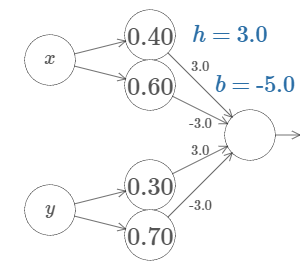
\includegraphics[width=0.24\linewidth]{./figures/ch4/tikz436}
	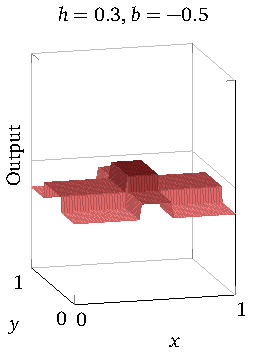
\includegraphics[width=0.24\linewidth]{./figures/ch4/3d/towerconstruction1}
	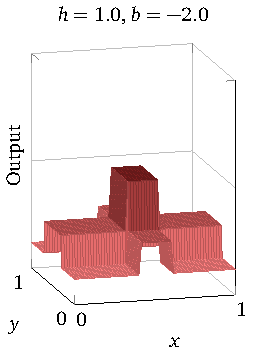
\includegraphics[width=0.24\linewidth]{./figures/ch4/3d/towerconstruction2}
	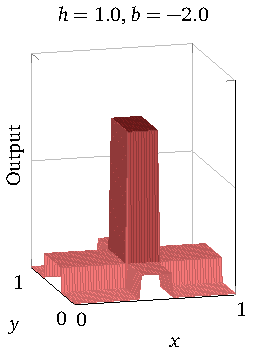
\includegraphics[width=0.24\linewidth]{./figures/ch4/3d/towerconstruction3}
\end{center}
With our initial parameters, the output looks like a flattened version of the earlier diagram, with its tower and plateau. To get the desired behaviour, we increase the parameter $h$ until it becomes large. That gives the if-then-else thresholding behaviour. Second, to get the threshold right, we'll choose $b\approx-3h/2$. Try it, and see how it works!

Here's what it looks like, when we use $h=10$:
\begin{center}
	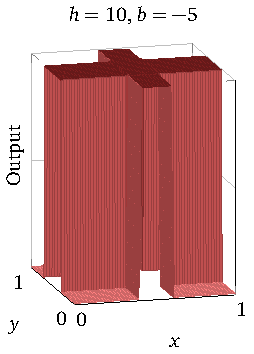
\includegraphics[width=0.24\linewidth]{./figures/ch4/3d/towerconstruction4}
	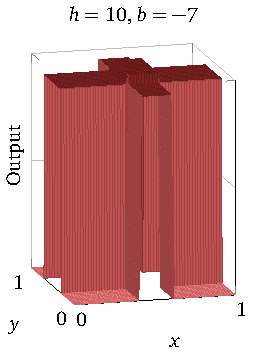
\includegraphics[width=0.24\linewidth]{./figures/ch4/3d/towerconstruction5}
	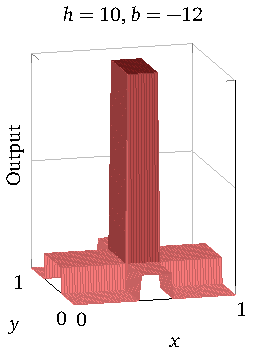
\includegraphics[width=0.24\linewidth]{./figures/ch4/3d/towerconstruction6}
	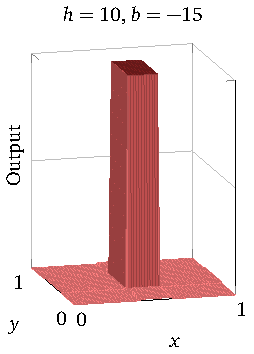
\includegraphics[width=0.24\linewidth]{./figures/ch4/3d/towerconstruction7}
\end{center}
Even for this relatively modest value of $h$, we get a pretty good tower function. And, of course, we can make it as good as we want by increasing $h$ still further, and keeping the bias as $b=-3h/2$.

Let's try gluing two such networks together, in order to compute two different tower functions. To make the respective roles of the two sub-networks clear I've put them in separate boxes, below: each box computes a tower function, using the technique described above. The graph on the right shows the weighted output from the second hidden layer, that is, it's a weighted combination of tower functions.
\begin{center}
	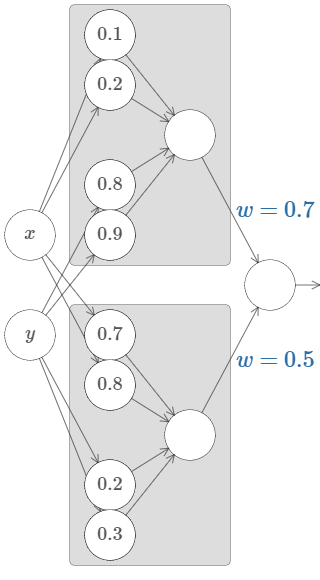
\includegraphics[width=0.24\linewidth]{./figures/ch4/tikz437}
	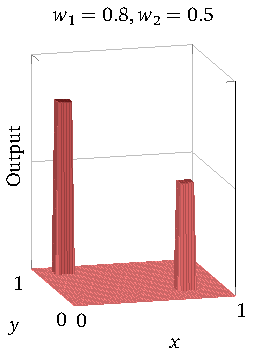
\includegraphics[width=0.24\linewidth]{./figures/ch4/3d/twotowers1}
	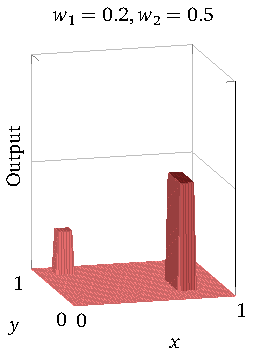
\includegraphics[width=0.24\linewidth]{./figures/ch4/3d/twotowers2}
	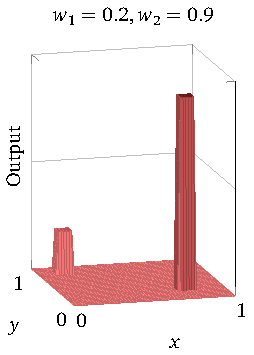
\includegraphics[width=0.24\linewidth]{./figures/ch4/3d/twotowers3}
\end{center}
%
%x=1y=1Weighted output
%
In particular, you can see that by modifying the weights in the final layer you can change the height of the output towers.

The same idea can be used to compute as many towers as we like. We can also make them as thin as we like, and whatever height we like. As a result, we can ensure that the weighted output from the second hidden layer approximates any desired function of two variables:
\begin{center}
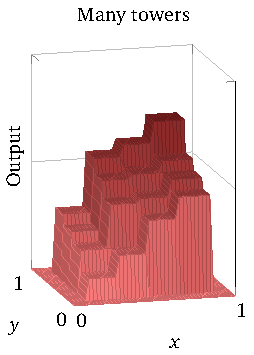
\includegraphics[width=0.32\linewidth]{figures/ch4/3d/manytowers2}
\end{center}
%\begin{lstlisting}
%ANIMATION
%\end{lstlisting}
%%
%x=1y=1Many towers
In particular, by making the weighted output from the second hidden layer a good approximation to $\sigma^{-1}\circ f$, we ensure the output from our network will be a good approximation to any desired function, $f$.

What about functions of more than two variables?

Let's try three variables $x_1,x_2,x_3$. The following network can be used to compute a tower function in four dimensions:
\begin{center}
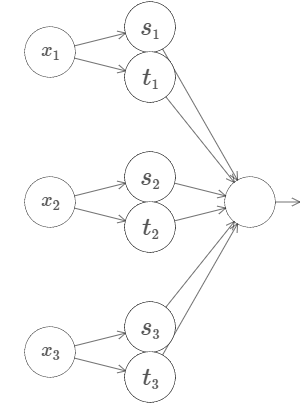
\includegraphics[width=0.35\linewidth]{figures/ch4/tikz441}
\end{center}
Here, the $x_1,x_2,x_3$ denote inputs to the network. The $s_1,t_1$ and so on are step points for neurons -- that is, all the weights in the first layer are large, and the biases are set to give the step points $s_1,t_1,s_2,\ldots$. The weights in the second layer alternate $+h$,$-h$, where $h$ is some very large number. And the output bias is $-5h/2$.

This network computes a function which is 1 provided three conditions are met: $x_1$ is between $s_1$ and $t_1$; $x_2$ is between $s_2$ and $t_2$; and $x_3$ is between $s_3$ and $t_3$. The network is 0 everywhere else. That is, it's a kind of tower which is 1 in a little region of input space, and 0 everywhere else.

By gluing together many such networks we can get as many towers as we want, and so approximate an arbitrary function of three variables. Exactly the same idea works in $m$ dimensions. The only change needed is to make the output bias $(-m+1/2)h$, in order to get the right kind of sandwiching behavior to level the plateau.

Okay, so we now know how to use neural networks to approximate a real-valued function of many variables. What about vector-valued functions $f(x_1,\ldots,x_m)\in R^n$? Of course, such a function can be regarded as just $n$ separate real-valued functions, $f^1(x_1,\ldots,x_m)$,$f^2(x_1,\ldots,x_m)$, and so on. So we create a network approximating $f^1$, another network for $f^2$, and so on. And then we simply glue all the networks together. So that's also easy to cope with.

\begin{exercize}{Problem}
\item We've seen how to use networks with two hidden layers to approximate an arbitrary function. Can you find a proof showing that it's possible with just a single hidden layer? As a hint, try working in the case of just two input variables, and showing that: (a) it's possible to get step functions not just in the x or y directions, but in an arbitrary direction; (b) by adding up many of the constructions from part (a) it's possible to approximate a tower function which is circular in shape, rather than rectangular; (c) using these circular towers, it's possible to approximate an arbitrary function. To do part (c) it may help to use ideas from a bit later in this chapter.
\end{exercize}
\section{Extension beyond sigmoid neurons}
We've proved that networks made up of sigmoid neurons can compute any function. Recall that in a sigmoid neuron the inputs $x_1,x_2,\ldots$ result in the output $\sigma$($\sum_jw_jx_j+b$), where $w_j$ are the weights, $b$ is the bias, and $\sigma$ is the sigmoid function:
\begin{center}
	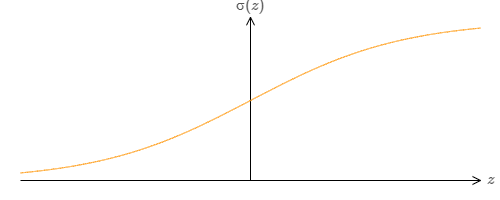
\includegraphics[width=0.7\linewidth]{figures/ch4/tikz451}
\end{center}
What if we consider a different type of neuron, one using some other activation function, $s(z)$:
\begin{center}
	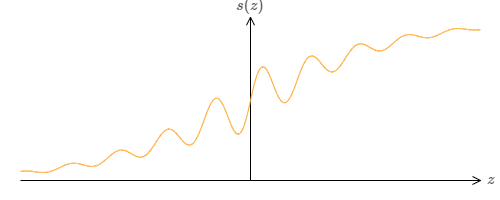
\includegraphics[width=0.7\linewidth]{figures/ch4/tikz452}
\end{center}
That is, we'll assume that if our neurons have inputs $x_1,x_2,\ldots$, weights $w_1,w_2,\ldots$ and bias $b$, then the output is $s(\sum_jw_jx_j+b)$.

We can use this activation function to get a step function, just as we did with the sigmoid. Try ramping up the weight in the following, say to $w=100$:

\begin{tikzpicture}[declare function = {sigma(\x) = 1/(1+exp(-\x)); neuron(\x) = sigma(\x)+0.2*sin(10*deg(\x))*exp(-abs(\x)); f(\x,\w,\b) = neuron(\w*\x+\b);}]
	\pgfplotsset{every axis legend/.append style={at={(1.03,1)},anchor=north west}}

		\begin{axis}[width=0.75\linewidth,height=0.45\linewidth,title={Output from neuron},axis x line=bottom,axis y line=left,xtick={0,1},ytick={0,1},xmax=1.05,ymax=1.05]
		%\addplot[blue!90!red,domain=0:1,samples=101]{f(x,9,-3)};
		\addplot[black,domain=0:0.2,samples=200]{f(x,100,-3)};
		\addplot[blue!90!red,domain=0:1,samples=200]{f(x,15,-3)};
		\addplot[blue!75!red,domain=0:1,samples=100]{f(x,8,-3)};
		\addplot[blue!50!red,domain=0:1,samples=100]{f(x,6,-3)};
		\addplot[blue!25!red,domain=0:1,samples=100]{f(x,4,-3)};
		\addplot[black,domain=0.2:1,samples=50]{1};
		%\addplot[blue!10!red,domain=0:1,samples=101]{f(x,3,-3)};
		\addlegendentry{$w=100, b = -3$}
		\addlegendentry{$w=15, b = -3$}
		%\addlegendentry{$w=9, b = -3$}
		\addlegendentry{$w=8, b = -3$}
		\addlegendentry{$w=6, b = -3$}
		\addlegendentry{$w=4, b = -3$}
		%\addlegendentry{$w=3, b = -3$}
		
	\end{axis}
\end{tikzpicture}

\begin{tikzpicture}[declare function = {sigma(\x) = 1/(1+exp(-\x)); neuron(\x) = sigma(\x)+0.2*sin(10*deg(\x))*exp(-abs(\x)); f(\x,\w,\b) = neuron(\w*\x+\b);}]
\pgfplotsset{every axis legend/.append style={at={(1.03,1)},anchor=north west}}
\begin{axis}[width=0.75\linewidth,height=0.45\linewidth,axis x line=bottom,axis y line=left,xtick={0,1},ytick={0,1},xmax=1.05,ymax=1.05]
	\addplot[blue!90!red,domain=0:1,samples=101]{f(x,6,-5)};
	%\addplot[blue!75!red,domain=0:1,samples=101]{f(x,6,-4)};
	\addplot[blue!50!red,domain=0:1,samples=101]{f(x,6,-3)};
	%\addplot[blue!25!red,domain=0:1,samples=101]{f(x,6,-2)};
	\addplot[blue!10!red,domain=0:1,samples=101]{f(x,6,-1)};
	\addlegendentry{$w=6, b = -5$}
	%\addlegendentry{$w=6, b = -4$}
	\addlegendentry{$w=6, b = -3$}
	%\addlegendentry{$w=6, b = -2$}
	\addlegendentry{$w=6, b = -1$}
\end{axis}
\end{tikzpicture}

\noindent Just as with the sigmoid, this causes the activation function to contract, and ultimately it becomes a very good approximation to a step function. Try changing the bias, and you'll see that we can set the position of the step to be wherever we choose. And so we can use all the same tricks as before to compute any desired function.

What properties does s(z) need to satisfy in order for this to work? We do need to assume that s(z) is well-defined as $z\to\infty$ and $z\to\infty$. These two limits are the two values taken on by our step function. We also need to assume that these limits are different from one another. If they weren't, there'd be no step, simply a flat graph! But provided the activation function s(z) satisfies these properties, neurons based on such an activation function are universal for computation.

\begin{exercize}{Problems}
\item Earlier in the book we met another type of neuron known as a rectified linear unit. Explain why such neurons don't satisfy the conditions just given for universality. Find a proof of universality showing that rectified linear units are universal for computation.
\item Suppose we consider linear neurons, i.e., neurons with the activation function $s(z)=z$. Explain why linear neurons don't satisfy the conditions just given for universality. Show that such neurons can't be used to do universal computation.
\end{exercize}
\section{Fixing up the step functions}
Up to now, we've been assuming that our neurons can produce step functions exactly. That's a pretty good approximation, but it is only an approximation. In fact, there will be a narrow window of failure, illustrated in the following graph, in which the function behaves very differently from a step function:
\begin{center}
	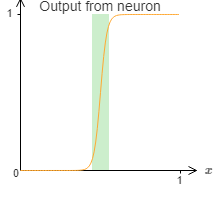
\includegraphics[width=0.4\linewidth]{figures/ch4/tikz453}
\end{center}
In these windows of failure the explanation I've given for universality will fail.

Now, it's not a terrible failure. By making the weights input to the neurons big enough we can make these windows of failure as small as we like. Certainly, we can make the window much narrower than I've shown above -- narrower, indeed, than our eye could see. So perhaps we might not worry too much about this problem.

Nonetheless, it'd be nice to have some way of addressing the problem.

In fact, the problem turns out to be easy to fix. Let's look at the fix for neural networks computing functions with just one input and one output. The same ideas work also to address the problem when there are more inputs and outputs.

In particular, suppose we want our network to compute some function, f. As before, we do this by trying to design our network so that the weighted output from our hidden layer of neurons is $\sigma^{-1}\circ f(x)$:
\begin{center}
	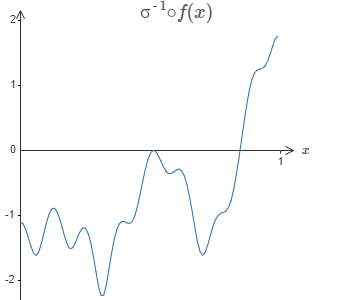
\includegraphics[width=0.6\linewidth]{figures/ch4/tikz454}
\end{center}
If we were to do this using the technique described earlier, we'd use the hidden neurons to produce a sequence of bump functions:
\begin{center}
	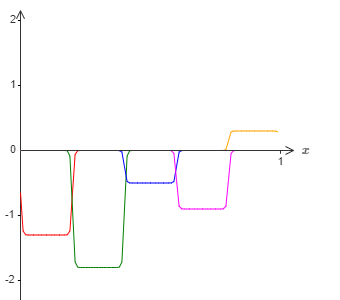
\includegraphics[width=0.4\linewidth]{figures/ch4/tikz455}
\end{center}
Again, I've exaggerated the size of the windows of failure, in order to make them easier to see. It should be pretty clear that if we add all these bump functions up we'll end up with a reasonable approximation to $\sigma^{-1}\circ f(x)$, except within the windows of failure.

Suppose that instead of using the approximation just described, we use a set of hidden neurons to compute an approximation to half our original goal function, i.e., to $\sigma^{-1}\circ f(x)/2$. Of course, this looks just like a scaled down version of the last graph:
\begin{center}
	\includegraphics[width=0.4\linewidth]{figures/ch4/tikz456}
\end{center}
And suppose we use another set of hidden neurons to compute an approximation to $\sigma^{-1}\circ f(x)/2$, but with the bases of the bumps \textit{shifted} by half the width of a bump:
\begin{center}
	\includegraphics[width=0.4\linewidth]{figures/ch4/tikz457}
\end{center}
Now we have two different approximations to $\sigma^{-1}\circ f(x)/2$. If we add up the two approximations we'll get an overall approximation to $\sigma^{-1}\circ f(x)$. That overall approximation will still have failures in small windows. But the problem will be much less than before. The reason is that points in a failure window for one approximation won't be in a failure window for the other. And so the approximation will be a factor roughly 2 better in those windows.

We could do even better by adding up a large number, $M$, of overlapping approximations to the function $\sigma^{-1}\circ f(x)/M$. Provided the windows of failure are narrow enough, a point will only ever be in one window of failure. And provided we're using a large enough number $M$ of overlapping approximations, the result will be an excellent overall approximation.

\section*{Conclusion}
The explanation for universality we've discussed is certainly not a practical prescription for how to compute using neural networks! In this, it's much like proofs of universality for NAND gates and the like. For this reason, I've focused mostly on trying to make the construction clear and easy to follow, and not on optimizing the details of the construction. However, you may find it a fun and instructive exercise to see if you can improve the construction.

Although the result isn't directly useful in constructing networks, it's important because it takes off the table the question of whether any particular function is computable using a neural network. The answer to that question is always ``yes''. So the right question to ask is not whether any particular function is computable, but rather what's a good way to compute the function.

The universality construction we've developed uses just two hidden layers to compute an arbitrary function. Furthermore, as we've discussed, it's possible to get the same result with just a single hidden layer. Given this, you might wonder why we would ever be interested in deep networks, i.e., networks with many hidden layers. Can't we simply replace those networks with shallow, single hidden layer networks?

\footnotetext{Chapter acknowledgments: Thanks to Jen Dodd and Chris Olah for many discussions about universality in neural networks. My thanks, in particular, to Chris for suggesting the use of a lookup table to prove universality. The interactive visual form of the chapter is inspired by the work of people such as Mike Bostock, Amit Patel, Bret Victor, and Steven Wittens.}

While in principle that's possible, there are good practical reasons to use deep networks. As argued in Chapter 1, deep networks have a hierarchical structure which makes them particularly well adapted to learn the hierarchies of knowledge that seem to be useful in solving real-world problems. Put more concretely, when attacking problems such as image recognition, it helps to use a system that understands not just individual pixels, but also increasingly more complex concepts: from edges to simple geometric shapes, all the way up through complex, multi-object scenes. In later chapters, we'll see evidence suggesting that deep networks do a better job than shallow networks at learning such hierarchies of knowledge. To sum up: universality tells us that neural networks can compute any function; and empirical evidence suggests that deep networks are the networks best adapted to learn the functions useful in solving many real-world problems.
\end{document}